\chapter{Introduction}

This chapter is based on the first chapter of \cite{magnusCombinatorialGroupTheory2004}. This chapter will be an introduction of what groups are and how they are generated.\\

We recall in group theory that a group $(G,\cdot)$ is a non-empty set $G$ of elements with a binary operation $\cdot$ for which the next axioms are satisfied:

\begin{itemize}
  \item \textbf{Closure:} For all $a,b \in G$, $c$ such that $a\cdot b = c$ implies that $c \in G$.

  \item \textbf{Associativity:} The operation $\cdot$ is associative, which means that for any elements $a,b,c \in G$:
    $$(ab)c = a(bc)$$

  \item \textbf{Identity element:} There exists an element of $G$ noted $1$ for which:

  $$a\cdot 1 = 1\cdot a = a$$

  \item \textbf{Inverse element:} For any $a \in G$ there exists an \textit{element} $a^{-1}$ for which:
  $$ a\cdot a^{-1} = a^{-1} \cdot a = 1 $$
\end{itemize}

We know two ways of defining a group; defining a \textit{symmetry} of a set and if it is presented by generators and relators.

\section{Symmetric groups}

\begin{definition}[Symmetric group]
The symmetric group on the set $G$ is the group whose elements are permutations of the elements of $G$ and its operation is the permutation composition. If $G = \{1,\dots, n$ we call it $S_n$. \cite{saganSymmetricGroup2001}.
\end{definition}

\begin{proposition}$S_n$ has order $n!$ and every group $G$ of order $n$ is a subgroup of $S_n$.
\end{proposition}

\subsection{Permutations}

Now that we know what symmetric groups are, we know that it's mainly based in permutations. In this subsection we define every operation on permutations used in these groups.


\begin{definition}[Two-line notation]
Given $i \in \{1,\dots,n\}$ and $\pi$ the permutation function we represent a permutation listing every elements of the set in two lines where in the first line we have the elements and the second one its image in the $\pi$ function:

\begin{equation}
  \begin{pmatrix}
   1 & 2 & 3 & 4 & 5 & \dots & i \\
   \pi(1) & \pi(2) & \pi(3) & \pi(4) & \pi(5) & \ & \pi(i)
 \end{pmatrix}
\end{equation}

\end{definition}


\begin{definition}[Cycle notation]Given $i \in \{1,\dots,n\}$ and $\pi$ the permutation function, the elements of the sequence $i, \pi(i), \pi^2(i),\dots$ cannot be distinct. Taking the power $p$ such that $\pi^p(i) = i$, we can note the permutation as the cycle:

\begin{equation}
  (i, \pi(i), \pi^2(i), \dots, \pi^{p-1}(i))
\end{equation}
\end{definition}

Which means that given a cycle $(i,j,k)$, the element $i$ is send to $j$, $j$ is sent to $k$ and $k$ is sent to $i$, cyclically, e.g. the permutation $23145$ of $n = \{1,2,3,4,5\}$ can be written with cycle notation as $(1,2,3)(4)(5)$. Remark that every element of the set has to be used.

\section{Presentation of groups}
\label{sec:pres_group}

In this section we show how a group can be defined by generators and relators:

\begin{definition}
  A group can be defined by:
  \begin{equation}
    Gr \cong \langle G | R\rangle
  \end{equation}

  being $G = \{a,b,c,\dots\}$ the set of \emph{generators} and $R = \{A,B,C,\dots\}$ the set of \emph{relators} or \emph{relations} such that every $X \in R$ is a word in $(G\cup G^{-1})^*$ such that $X = 1$.
\end{definition}

For example, the dihedral group $D_n$ has the next presentation where $q$ is a rotation and $r$ a reflection:

$$D_n \cong \langle \{q,r\} | \{r^2, q^n, rqrq\} \rangle$$

\chapter{Coxeter groups}
In this chapter, we explain the interest and motivation of coxeter groups by analysing a symmetric group. The main example of this chapter will be the symmetric group $S_3$. This group can be defined in three ways.

\begin{figure}
  \begin {center}
  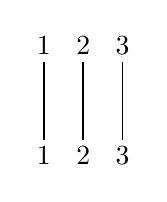
\begin{tikzpicture}
  	% general shift to north east
    \draw (0,1+0.2) node {$1$};
    \draw (0.5,1+0.2) node {$2$};
    \draw (1,1+0.2) node {$3$};
  	\draw[semithick] (0,0) -- (0,1);% first line
  	\draw[semithick] (0.5,0) -- (0.5,1);% second line
  	\draw[semithick] (1,0) -- (1,1);% third line
    \draw (0,-0.2) node {$1$};
    \draw (0.5,-0.2) node {$2$};
    \draw (1,-0.2) node {$3$};
  \end{tikzpicture}

  \caption{The wiring diagram for the permutation $123$.}
  \end{center}
\label{fig:wiring}
\end{figure}

\begin{figure}
  \begin {center}
  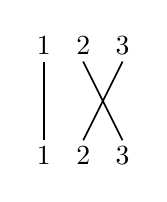
\begin{tikzpicture}
    % general shift to north east
    \draw (0,1+0.2) node {$1$};
    \draw (0.5,1+0.2) node {$2$};
    \draw (1,1+0.2) node {$3$};
    \draw[semithick] (0,0) -- (0,1);% first line
    \draw[semithick] (0.5,0) -- (1,1);% second line
    \draw[semithick] (1,0) -- (0.5,1);% third line
    \draw (0,-0.2) node {$1$};
    \draw (0.5,-0.2) node {$2$};
    \draw (1,-0.2) node {$3$};
  \end{tikzpicture}
  \caption{The wiring diagram for the permutation $132$.}
  \end{center}
\label{fig:wiring_23}
\end{figure}

\begin{figure}
  \begin {center}
  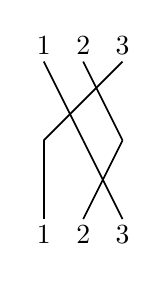
\begin{tikzpicture}
    % general shift to north east
    \draw (0,2+0.2) node {$1$};
    \draw (0.5,2+0.2) node {$2$};
    \draw (1,2+0.2) node {$3$};
    \draw[semithick] (0,0) -- (0,1);% first line
    \draw[semithick] (0,1) -- (1,2);% first line
    \draw[semithick] (0.5,0) -- (1,1);% second line
    \draw[semithick] (0.5,1) -- (0,2);% second line
    \draw[semithick] (1,0) -- (0.5,1);% third line
    \draw[semithick] (1,1) -- (0.5,2);% third line
    \draw (0,-0.2) node {$1$};
    \draw (0.5,-0.2) node {$2$};
    \draw (1,-0.2) node {$3$};
  \end{tikzpicture}

  \caption{The wiring diagram for the permutation composition $132 \circ 231$.}
  \end{center}
\label{fig:wiring_compo}
\end{figure}


\begin{figure}
  \begin{center}
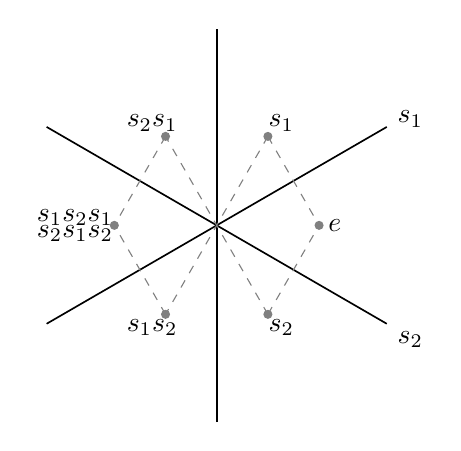
\begin{tikzpicture}
	% general shift to north east
	\draw[semithick] (0,-2.5) -- (0,2.5);% center line
  \draw[semithick] (-2.16,1.25) -- (2.16,-1.25);% first symmetry
  \draw[semithick] (2.16,1.25) -- (-2.16,-1.25);% second symmetry

  \def\offX{0.65}
  \def\offY{1.13}
	\draw[dashed,color=gray] (0+\offX,0+\offY) -- (0.65+\offX,-1.13+\offY);% e to s_1
  \draw[dashed,color=gray] (0+\offX,0-\offY) -- (0.65+\offX,-1.13+\offY);% e to s_2
	\draw[dashed,color=gray] (0+\offX,0+\offY) -- (0-\offX,0-\offY);% s_1 to s_1s_2
  \draw[dashed,color=gray] (0+\offX,0-\offY) -- (0-\offX,0+\offY);% s_2 to s_2s_1
  \draw[dashed,color=gray] (0-\offX,0+\offY) -- (-1.3,0);% s_1s_2 to s_1s_2s_1
  \draw[dashed,color=gray] (0-\offX,0-\offY) -- (-1.3,0);% s_2s_1 to s_2s_1s_2

  \draw [fill=gray, color=gray](1.3,0) circle (0.05);
  \draw [fill=gray, color=gray](-1.3,0) circle (0.05);
  \draw [fill=gray, color=gray](0+\offX,0+\offY) circle (0.05);
  \draw [fill=gray, color=gray](0-\offX,0+\offY) circle (0.05);
  \draw [fill=gray, color=gray](0+\offX,0-\offY) circle (0.05);
  \draw [fill=gray, color=gray](0-\offX,0-\offY) circle (0.05); % s_1s_2

  % axis
  \def\offAx{0.2}
  \draw (2.16+\offAx+0.1,-1.25-\offAx) node {$s_2$};
  \draw (2.16+\offAx+0.1,+1.25+\offAx-0.1) node {$s_1$};

  \draw (1.5,0) node {$e$};
  \draw (-1.8,0+0.1) node {$s_1s_2s_1$};
  \draw (-1.8,0-0.1) node {$s_2s_1s_2$};
  \draw (0+\offX + 0.17,0+\offY + 0.17) node {$s_1$};
  \draw (0+\offX + 0.17,0-\offY - 0.17) node {$s_2$};
  \draw (0-\offX - 0.17,0+\offY + 0.17) node {$s_2s_1$};
  \draw (0-\offX - 0.17,0-\offY - 0.17) node {$s_1s_2$};
\end{tikzpicture}
\end{center}
\caption{Geometrical representation of $S_3$. The grey dotted lines represent the reflection applied between two points.}
\label{fig:geoS3}
\end{figure}

\begin{itemize}
  \item Combinatorial: Given a cyclic noted permutation we can represent it as a \emph{wiring diagram}.

  For example, for the permutation $123$ we have the following wire diagram:
  \item Algebraic: Presentation of groups as seen in section \ref{sec:pres_group}.
  \begin{equation}\label{equation donnant la form explicite de pi}
  \begin{split}
  S_3 \cong \langle \{s_1, s_2\} | s_1s_2s_1 &= s_2s_1s_2 , s_1^2 = e, s_2^2 = e,\\
   &(s_1s_2)^3 = s_1s_2s_1s_2s_1s_2 = e\} \rangle
  \end{split}
  \end{equation}

  \item Geometrical: We can represent geometrically a coxeter group by reflections. In figure \ref{fig:geoS3} you can see a geometrical representation of $S_3$ where $s_1$ and $s_2$ are the generators of $S_3$ and also reflections on the plane.

  If you see the figure you can remark that $s_1s_2s_1 = s_2s_1s_2$, $s_1^2 = e$ and $s_2^2$; $S_3$ is a coxeter group.
\end{itemize}

\section{Coxeter groups}

In this section we define the mathematical objects that represent coxeter groups. $S$ being a finite set:

\begin{definition}
  A \emph{coxeter matrix} $m : S\times S \to \{1,2,\dots,\infty\}$ such that:
  \begin{enumerate}
    \item $m(s,s') = 1 \ \ \forall s \in S$
    \item $m(s,s') = m(s', s) \ \ \forall s \in S$
    \item $m(s,s') > 1\ \ \ \text{if}\  s \neq s'$
  \end{enumerate}
\end{definition}

\begin{definition}
  A \emph{coxeter diagram} is a graph where the set of vertices are the elements of $S$ and
  the labelled edges are such that:
  \begin{enumerate}
    \item if $m(s,s') = 2$:\ \dynkin[labels={s},label macro/.code={#1}]{A}{1}
                      \dynkin[labels={s'},label macro/.code={#1}]{A}{1}
    \item if $m(s,s') = 3$:  \dynkin[labels={s,s'},label macro/.code={#1}]{A}{2}
    \item if $m(s,s') \geq 4$: \dynkin[labels={s,s'},label macro/.code={#1}]{A}{2} where the label of the edge is $m(s,s')$.
  \end{enumerate}

  where $m$ is the coxeter matrix.
\end{definition}

\begin{example}
	If we have a coxeter matrix $m$:
    \begin{equation}
      m =
    \begin{bmatrix}
    1 & 3 & 2\\
    3 & 1 & 4\\
    2 & 4 & 1\\
    \end{bmatrix}
    \end{equation}

  where the line or column $i$ corresponds to the generator $s_i$ of the coxeter group. Then the related coxeter diagram can be drawn like this:

  \center{\dynkin[Coxeter, labels={s_1, s_2, s_3}]{B}{3}}
\end{example}

Given the definition of $m$, we can now define formally a coxeter group.

\begin{definition}
A \emph{coxeter group} is a group with the following presentation:

\begin{equation}
  \langle S\  |\  (s, s')^{m(s,s')} = e, \forall s, s' \in S\} \rangle
\end{equation}
where $S$ si a group and $m$ the coxeter matrix with $m(s,s') < \infty$.

\end{definition}

\begin{example}
  The symmetric group $S_n$ can be represented with the following coxeter diagram:
  \begin{center}
    \dynkin[Coxeter, labels={s_1, s_2, s_{n-1}, s_n}, edge length=.50cm]{A}{}
  \end{center}

  because for every $i < n$, we have that $s_is_{i+1}s_is_{i+1} = e$, so $(s_is_{i+1})^2 = e$, which means that
  $m(s_i, s_{i+1}) = 2$ for every $i < n$.
\end{example}

\begin{definition}
  The tuple $(W,S)$ is a coxeter system where $W$ is a coxeter group and $S$ a group of generators.
\end{definition}

\begin{figure}
  \begin {center}
  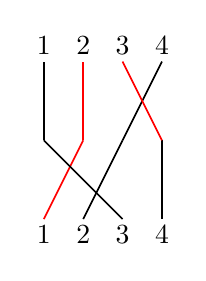
\begin{tikzpicture}
    \draw (0,2+0.2) node {$1$};
    \draw (0.5,2+0.2) node {$2$};
    \draw (1,2+0.2) node {$3$};
    \draw (1.5,2+0.2) node {$4$};
    \draw[semithick, color=red] (0,0) -- (0.5,1);% first line
    \draw[semithick, color=red] (0.5,1) -- (0.5,2);% first line
    \draw[semithick] (0.5,0) -- (1,1);% second line
    \draw[semithick] (0,1) -- (0,2);% second line
    \draw[semithick] (1,0) -- (0,1);% third line
    \draw[semithick] (1,1) -- (1.5,2);% third line
    \draw[semithick] (1.5,0) -- (1.5,1);% fourth line
    \draw[semithick, color=red] (1.5,1) -- (1,2);% fourth line
    \draw (0,-0.2) node {$1$};
    \draw (0.5,-0.2) node {$2$};
    \draw (1,-0.2) node {$3$};
    \draw (1.5,-0.2) node {$4$};
  \end{tikzpicture}
  \caption{The wiring diagram for the permutation  $3\bar{1}24 \circ 1\bar{2}\bar{4}3$. You can see that there is a permutation that changes its sign two times.}
  \end{center}
\label{fig:wiring_snB}
\end{figure}

We introduce the hyperoctahedral group $S_n^B$ being the group of signed permutations of $\big[n\big] := \{1, 2, \dots, n\}$. The group set is $\{1,2,\dots,m,\bar{1}, \bar{2},\dots, \bar{n}\}$. We have a new generator $t$, that will change the sign of an element. In figure \ref{fig:wiring_snB} you can see an example of permutations withing this group. This is a coxeter group and its diagram is:

\begin{center}
  \dynkin[Coxeter, labels={s_n, s_{n-1}, s_{n-2},s_2,s_1, t}, edge length=.50cm, gonality=n ]{B}{}
\end{center}

Given a coxeter system $(W,S)$, we can then define $T := \{wsw^{-1} |\ s\in S, w \in W\} \subseteq W$ where $s$ are simple reflections. Now we can define $\pi$.

\begin{definition}
  Given $W \to S_T^B$ and $w \to \pi_w$ with $t\in T$ and $s\in S$:

  \begin{equation}
    \pi_s(t) := \left \{
    \begin{array}{c @{} c}
        -s \quad &\text{if } t = s \\
        sts \quad &\text{if } t \neq s \\
    \end{array}\right.
  \end{equation}
\end{definition}

This application is a bijection because its inverse is itself ($\pi_s(\pi_s(s)) = s$):

\begin{equation}
  \pi(\pi_s(t)) = \left \{
  \begin{array}{c @{} c}
      \pi_s(-s) \quad &\text{if } t = s \\
      \pi_s(tsts) \quad &\text{if } t \neq s \\
  \end{array}\right.
\end{equation}

We clearly see that $\pi_s(sts) = s(sts)s = t$ and $\pi_s(-s) = -\pi_s(s) = -s$.

%\begin{equation}

%\end{equation}
